% =====================================================================================
% Manuscript for IEEE Transactions on Pattern Analysis and Machine Intelligence (TPAMI)
% DRAFT 2026-10-20. Build:  latexmk -pdf main.tex   (in paper/)
% Figures: paper/figures/make_figures.py  (all numbers it prints are in figures/numbers.txt)
% \pending{...} marks text that waits on data or decisions; it prints in red.
% =====================================================================================
\documentclass[10pt,journal,compsoc]{IEEEtran}

\usepackage[nocompress]{cite}
\usepackage{amsmath,amssymb}
\usepackage{graphicx}
\usepackage{booktabs}
% minimal unit macros (this MiKTeX's siunitx fails inside \maketitle)
\newcommand{\SI}[2]{#1\,#2}
\newcommand{\si}[1]{#1}
\newcommand{\SIrange}[3]{#1--#2\,#3}
\newcommand{\micro}{\ensuremath{\mu}}
\newcommand{\nano}{n}\newcommand{\milli}{m}\newcommand{\mega}{M}
\newcommand{\second}{s}\newcommand{\hertz}{Hz}\newcommand{\metre}{m}
\newcommand{\percent}{\%}
\usepackage{xcolor}
\usepackage{tikz}
\usetikzlibrary{arrows.meta,positioning,fit,backgrounds}
\usepackage{url}
\usepackage[T1]{fontenc}

\newcommand{\pending}[1]{\textcolor{red}{[#1]}}
\newcommand{\us}{\,\si{\micro\second}}

\begin{document}

\title{Bring Your Own Projector: An FPGA Camera Inside the HDMI Path\\
for Genlocked Structured Light and Projector Profiling}

\author{Daniel~L.~Lau% \pending{IEEE membership grade?}
\IEEEcompsocitemizethanks{\IEEEcompsocthanksitem D.\,L.~Lau is with the Department of
Electrical and Computer Engineering, University of Kentucky, Lexington, KY 40506, USA.\protect\\
E-mail: dllau@uky.edu}}

\markboth{IEEE Transactions on Pattern Analysis and Machine Intelligence}%
{Lau: Bring Your Own Projector}

\IEEEtitleabstractindextext{%
\begin{abstract}
Structured-light illumination (SLI) assumes that the camera integrates exactly one projected
pattern per exposure. With an off-the-shelf digital light processing (DLP) projector that
assumption is rarely checked: the projector re-times the video it receives, delays it by an
unknown latency, and paints each frame as an interleaved sequence of colour-LED and bit-plane
pulses whose timing is undocumented. We present a ``bring your own projector'' (BYOP) camera in
which a field-programmable gate array sits inline on the HDMI cable between a PC and an
unmodified projector. The same device reads the projector's EDID and drives it in a mode it
advertises, generates resolution-adaptive phase-shift patterns on the fly, triggers a
global-shutter PYTHON~1300 sensor at a programmable delay from the projected vertical sync with
\SI{10}{\nano\second} resolution, and queues triggers so that patterns advance at the full video
rate even when the delay exceeds a frame. Because the device controls both the picture and the
shutter, it can also measure the projector: stepping a \SI{4.875}{\micro\second} exposure across
a five-frame impulse sequence recovers the light the projector emits against time, which we
use to place the exposure, to decompose white into its red, green and blue LED pulses, and to
map the light that leaks into an exposure from the neighbouring patterns. On an Optoma ML750ST
at \SI{120}{\hertz} we find a one-frame latency and a train of separate red, green and blue LED pulses whose
filtered decomposition explains white with $R^2=0.9988$, and an exposure window that captures
\SI{95.6}{\percent} of a frame's light (\SI{99.2}{\percent} at the sensor's longest exposure);
light before the window depends on the previous pattern in one part and on the next pattern in
another. \pending{3D results: how much profiling and leakage correction improve phase and depth
error.}
\end{abstract}

\begin{IEEEkeywords}
Structured light, phase measuring profilometry, projector--camera systems, DLP, genlock,
FPGA, temporal characterization.
\end{IEEEkeywords}}

\maketitle
\IEEEdisplaynontitleabstractindextext
\IEEEpeerreviewmaketitle

% =====================================================================================
\section{Introduction}
\label{sec:intro}

% ---- 1. What structured light is, and how it differs from other 3D imaging ----------
\IEEEPARstart{S}{tructured} light illumination (SLI) refers to a method of 3D scanning that
uses a projector to project a series of light striped patterns such that a camera can
reconstruct depth based on the warping of the patterns over the target object's
surface~\cite{salvi2004pattern,geng2011tutorial,zuo2018phase}. In this way, the projector takes
the place of the second camera in a stereo pair, and the correspondence between a camera pixel
and a projector row or column is established by the projected patterns rather than by the
texture of the scene.

Passive stereo vision, by comparison, must find correspondences from
scene texture and fails on surfaces that have none~\cite{scharstein2002taxonomy}, while
time-of-flight (ToF) cameras measure depth directly from the round-trip time of modulated light
but at a lower lateral resolution and with depth errors caused by multi-path
reflections~\cite{hansard2012tof}. Laser line scanners, also based on triangulation, measure a
single profile per captured image~\cite{blais2004review}.

% ---- 2. It is a scanning process: motion is the enemy, so scan fast --------------------
Examples of SLI include single pattern techniques which project a static pattern from which a 3D
reconstruction can be made from a single snapshot~\cite{takeda1983fourier,geng2011tutorial}.
Multiple pattern SLI scanners, alternatively, project a series of patterns, trading temporal
resolution for spatial resolution such that each pixel can be independently processed from its
neighbors to produce a single point for each pixel in the camera. In phase measuring
profilometry (PMP), the projector coordinate of each pixel is encoded through phase modulation
over a minimum of three patterns, with multi-frequency schemes requiring
more~\cite{liu2010dualfreq,zuo2018phase}.

As a scanning process, multiple pattern SLI assumes that
the target object is stationary for the duration of the scan; when the object moves, the
samples recorded at a pixel come from different surface points, and the reconstruction suffers
from ripple and decoding errors~\cite{weise2007fast,zhang2018review}. For this reason, it is
desirable for the pattern sequence to run as fast as possible.

% ---- 3+4. Cameras cap the useful rate; light engines vs commodity projectors -----------
In practice, the camera limits the scan rate since each pattern must be captured in its own
image. Machine vision cameras with megapixel global-shutter sensors operate at around
\SI{200}{fps}, and the PYTHON~1300 sensor used in this paper operates at up to \SI{210}{fps} at
full resolution. DLP light engines built for structured light display binary patterns at tens
of thousands of patterns per second, a rate that such cameras cannot use, and they are either
expensive or dim (Section~\ref{sec:rw_engines}).

The scan rate is further limited by the light output of the projector and by the bandwidth
between the camera and the host computer. A projector with a low lumen output requires a longer
exposure to collect the same signal, and since each exposure must end before the next pattern's
exposure begins, the exposure time sets a lower bound on the time per pattern. At the same time,
every image must be transferred to the host: a $1280\times1024$ image at 10 bits per pixel is
\SI{1.64}{MB}, so \SI{120}{fps} requires \SI{197}{MB/s} of sustained bandwidth between the camera
and the host. A structured light scanner is therefore limited both by its exposure, and through
the exposure by its projector's light output, and by the bandwidth of its link to the host.
Low light output also rules out a simple remedy for the color processing of commodity projectors
described in Section~\ref{sec:rw_electronics}: projecting a single color and placing a matching
color filter on the camera lens. A filter that passes one LED of an RGB projector rejects the
light of the other two, and so it requires a still longer exposure for the same signal.

For these reasons, commodity projectors are an attractive alternative. ``3D-ready'' DLP
projectors accept \SI{120}{\hertz} video and can emit more than 1500 lumens, and if a light
output below 1000 lumens is acceptable, then LED projectors can be used, whose LED lifetimes of
tens of thousands of hours make them practical for industrial applications
(Section~\ref{sec:rw_engines}).

% ---- 5. Commodity projectors are hard to set up: no stored patterns, no GPIO -----------
Commodity projectors are, however, difficult to integrate into a 3D scanner. A commodity
projector cannot store a static set of patterns in hardware, so every pattern must be sent over
the video cable by a host computer whose graphics output makes no guarantee as to when each
frame is delivered. A commodity projector also cannot be slaved to a camera acting as master
through general purpose input/output (GPIO), nor can it trigger a camera, as structured light
light engines do~\cite{barreto2011dlp}. Of the published scanners built on commodity projectors
(Section~\ref{sec:rw_sync}), only that of Yu
\emph{et~al.}~\cite{yu2019dualspie,yu2020dualprojector} uses a controller fully interfaced between
the HDMI video signal and the GPIO trigger of the camera.

% ---- 6. The BYOP camera (from the press release) ---------------------------------------
The \emph{bring your own projector} (BYOP) machine vision camera was developed to control an
unmodified projector through its HDMI input~\cite{lau2026byop}, and it follows from the
structured light smart camera for spatial augmented reality applications of Ruffner
\emph{et~al.}~\cite{ruffner2019smartcamera}. The BYOP camera is a
global-shutter machine vision camera, streaming full frames over USB~3.0, with an HDMI receiver
and transmitter integrated on the same FPGA. Video from a host computer enters the camera and
passes through to the projector, so the camera sits in the video path rather than beside it and
knows what is being projected and when.

When a host computer drives the display, the camera
either passes the host's pixels through untouched and, using the top-left pixel method of
Yu~\cite{yu2019dissertation}, triggers only when the top-left pixel of the incoming
frame changes, or
replaces the host's pixels with structured light patterns of its own. When no host is attached,
the camera reads the projector's EDID, drives the projector at a mode the projector advertises,
generates its own pattern sequence, and triggers the sensor at a programmable delay after each
vertical sync it transmits, at up to \SI{120}{\hertz}. No trigger box, frame grabber, or
synchronization cabling is needed, and because the HDMI path runs through the camera, multiple
BYOP cameras can be daisy-chained on a single projector.

% ---- 7. Commodity projectors are designed for viewers, which causes problems for SLI ---
Controlling when a frame is sent to the projector does not, by itself, control when or how the
projector emits the light of that frame. Commodity projectors are designed to produce a
compelling display for a human viewer watching movies, and the processing between the HDMI input
and the emitted light serves that purpose rather than measurement. That processing delays each
frame by an input lag that depends on the display mode, renders a constant input level as a
temporal sequence of mirror states, applies a nonlinear tone curve, and can redistribute the RGB
input among illumination components that the HDMI signal cannot address independently
(Section~\ref{sec:rw_electronics}).

An RGB LED projector also creates a problem of its own for SLI. The white pattern is the sum of
three patterns, one from each LED, and a pixel of a monochrome camera records each of them
weighted by the reflectance of the surface in that LED's band, so that a green surface returns
mostly the green pattern and a blue surface mostly the blue. If the three LEDs produce the same
phase, the recorded phase is independent of the surface color. If they do not, because the LEDs
have different tone curves or because the exposure collects a different share of each LED's
light, then each pixel records a mixture of phases whose balance depends on its color, which is
the same form as the multi-path interference studied by Zhang
\emph{et~al.}~\cite{zhang2019bimodal,zhang2024bimodalps}, and the error cannot be removed by a
calibration made under the combined RGB light. Each LED must therefore be, by itself, a correct
SLI projector that produces the same phase as the other two.

% ---- 8. What this paper does -----------------------------------------------------------
This being the case, this paper studies the profiling of an LED commodity projector through the
BYOP camera, with the aim of compensating the HDMI signal so as to minimize the distortion caused
by the projector's electronics while achieving a \SI{120}{\hertz} scan rate.

\subsection{Contributions}
This paper is the first to describe the BYOP camera, and so the first contribution is the camera
itself, implemented on a single Xilinx Artix-7 FPGA. On the video side, the FPGA includes an HDMI
receiver that recovers the pixel clock of the incoming video by measuring its frequency and
selecting the matching clock-recovery band, such that it tracks the spread-spectrum clocks of
graphics cards, and an HDMI transmitter that either forwards the host's video or replaces it with
patterns generated on the FPGA. The FPGA reads the projector's EDID over the display data channel
and serves the host a merged EDID listing only the modes that both the projector and the camera
support.

With no host attached, the FPGA reprograms its own pixel clock at run time and selects,
from a table of 14 video modes, the fastest mode that the projector's EDID advertises, up to
1280$\times$1024 at \SI{60}{\hertz} or 800$\times$600 at \SI{120}{\hertz}. The on-board pattern
generator produces PMP patterns at three spatial frequencies in a fixed $1{:}6{:}36$ ratio with
eight phase shifts each, plus a flat full-field pattern, with the periods recomputed for the
resolution of each video mode, and passes every pattern through a 256-entry lookup table that
can be loaded from the host.

On the camera side, the FPGA triggers the PYTHON~1300 sensor at a
delay after the vertical sync of the video it transmits, programmable in \SI{10}{\nano\second}
steps. In the controller of Yu \emph{et~al.}~\cite{yu2020dualprojector}, the camera trigger
waited out the trigger delay and the exposure before the next frame could be handled, so the
fastest frame period was the trigger delay plus the exposure. The BYOP camera instead holds
triggers in a 32-entry queue of absolute fire times, stacking a new trigger at every vertical
sync while earlier ones are still pending, so that the frame period is limited only by the
exposure and a delay longer than one frame period still yields one image per projected frame.

The FPGA
limits the exposure to the frame period less the sensor's readout gap, receives the sensor's four
LVDS lanes at \SI{720}{Mbps}, buffers frames in DDR3 memory, and streams them to the host over
USB~3.0. In pass-through mode, the FPGA
samples the top-left pixel of every incoming HDMI frame and triggers the camera when that value
changes, and it writes the sampled value into the header of the captured frame, so that the host
can match each captured image to the pattern that was displayed. The header also carries the
mean intensity of a $16\times16$ pixel region of interest computed on the FPGA, which allows the
projector profiling of this paper to run without transferring images.

While this paper limits its discussion to a single LED projector, the Optoma ML750ST, we note
that the profiling procedure requires nothing from the projector other than an HDMI input, and so
it can be applied to any projector that the BYOP camera can drive. Using the BYOP camera's own
sensor, we sweep a \SI{4.875}{\micro\second} exposure across a five-frame impulse sequence to
measure the light emitted by the projector against time, from which we derive the projector's
latency, the timing of its LED pulses, and the exposure window that collects the most light from a
single video frame.

By repeating the sweep through red, green, and blue filters, we test whether
the projector's white output contains any interval during which two LEDs are on at once, which
determines whether the three channels of the HDMI signal fully control the emitted light, and we
measure the timing of each LED's light separately, which is the first requirement for the three
LEDs to produce the same phase. \pending{Per-LED phase test: scan a flat target through each
filter and compare the three phase maps.}

We
further measure the light that reaches the camera before the exposure window opens, and by means
of two-dimensional maps over pairs of gray levels, separate the light arriving from the previous
pattern from the light arriving from the pattern being captured. \pending{Compensation of
the HDMI signal from these measurements, and its effect on phase and depth error.}


% =====================================================================================
\section{Related Work}
\label{sec:related}

This section reviews the patterns of SLI and the projection hardware that displays them, then the ways that cameras
have been synchronized with commodity projectors, the FPGA cameras that use the same sensor as
the BYOP camera, the processing inside a projector that stands between its video input and its
light, and finally multi-path, the class of errors to which that processing contributes.

\subsection{Structured light and phase shifting}
Pattern codification strategies for SLI are surveyed by Salvi
\emph{et~al.}~\cite{salvi2004pattern} and by Geng~\cite{geng2011tutorial}, and phase-shifting
algorithms by Zuo \emph{et~al.}~\cite{zuo2018phase}. Liu \emph{et~al.}~\cite{liu2010dualfreq}
combine a high and a low spatial frequency in each pattern to unwrap phase with fewer patterns,
and Liu \emph{et~al.}~\cite{liu2010gamma} model the periodic phase error caused by the
projector's gamma. The pattern generator of the BYOP camera uses three spatial frequencies in a
fixed $1{:}6{:}36$ ratio, and it carries a lookup table in the pattern path so that the
projector's tone curve can be corrected before the patterns are sent.

High-speed SLI systems avoid the limits of video projection by displaying binary patterns
directly on a DMD. Zhang and Huang~\cite{zhang2006realtime} as well as Zhang
\emph{et~al.}~\cite{zhang2010superfast} use this approach for real-time and superfast phase
shifting, and Lei and Zhang~\cite{lei2009defocus} defocus the projector so that binary patterns
blur into sinusoids. Gong and Zhang~\cite{gong2010ultrafast} apply binary defocusing with an
off-the-shelf DLP projector. A review of these methods is given by Zhang~\cite{zhang2018review}. These systems depend on
projection hardware that exposes the DMD directly, which brings us to the light engines built
for that purpose.

\subsection{Light engines and commodity projectors}
\label{sec:rw_engines}
The DLP chipsets designed for high-speed pattern display operate far faster than any camera that
watches them. The DLPC410 controller drives the DLP7000 digital micromirror device (DMD) at up
to 23\,000 binary patterns per second over the full array, and at up to 48\,000 binary patterns
per second in its LOAD4 mode, which loads the same data into groups of four rows and so reduces
the vertical resolution by a factor of four~\cite{ti_dlpc410,ti_dlp7000}. Either rate exceeds the
frame rate of a megapixel machine vision camera by more than two orders of magnitude. Barreto
describes the structured light modes, stored pattern sequences, and trigger outputs of TI's
development kits~\cite{barreto2011dlp}; industrial light engines and development kits are
either very expensive or have a low lumen output \pending{cite: price of an industrial engine;
lumens of a DLP LightCrafter}.

Commodity projectors make the opposite trade, displaying patterns at a rate that machine vision
cameras can match. ``3D-ready'' DLP projectors, built for shutter-glass stereo viewing, accept \SI{120}{\hertz}
video and can have light outputs above 1500 lumens. As an example, ProjectorCentral measured
2494 lumens from the 3D-ready BenQ W600 in its brightest mode, and 1748 lumens in its standard
mode~\cite{pc_benq_w600}. The Optoma ML750ST used in this paper is an LED DLP projector with
individual red, green, and blue LEDs and a rated LED life of 20\,000 hours, and it accepts
800$\times$600 video at \SI{120}{\hertz}~\cite{optoma_ml750st,pc_ml750st_specs}.

Optoma rates the ML750ST at 700 lumens, a figure that ProjectorCentral reports as the perceived
equivalent of a lamp projector's ANSI lumens rather than a measured light output;
ProjectorCentral measured 490 lumens in the ML750ST's brightest mode and 322 lumens in its
cinema mode~\cite{pc_ml750st_review}. ProjectorCentral also lists the ML750ST's input lag, the
delay between the arrival of a frame at the HDMI input and its appearance on screen, as
\SI{16.5}{\milli\second} for 1080p video at \SI{60}{\hertz}~\cite{pc_ml750st_specs}.

We further note that faster scan rates are available from commodity 4K DLP projectors. TI's
0.47-inch 4K UHD DMD has an array of $1920\times1080$ micromirrors and displays a
$3840\times2160$ image by shifting the image among four positions with an optical actuator
(four-way XPR), and the chipsets built on this DMD accept 4K UHD video at \SI{60}{\hertz} or
1080p video at \SI{240}{\hertz}~\cite{ti_dlp471te,ti_dlpc6540}. An SLI scanner built around a
commodity 4K DLP projector could therefore scan at \SI{240}{\hertz}; such a scanner has not yet
been demonstrated. Whatever its rate, a commodity projector accepts patterns only through its
video input and offers no trigger, so a scanner built on one must synchronize its camera by
other means.

\subsection{Synchronizing commodity projectors and cameras}
\label{sec:rw_sync}
Examples of how to deal with this lack of synchronization include
Wilm \emph{et~al.}~\cite{wilm2014calibration}, who insert fixed pauses between pattern
presentation and image capture to accommodate buffering in the graphics card and projector, as
well as Petkovi\'c \emph{et~al.}~\cite{petkovic2016software}, who use the vertical blanking
interval of the video output as a timing reference and estimate the combined projector--camera
delay from captured images. Moreno \emph{et~al.}~\cite{moreno2015unsync} take the approach of
operating projector and camera independently and synthesizing, from the unsynchronized images,
the images that a synchronized system would have captured. Zuo
\emph{et~al.}~\cite{zuo2012highspeed}, alternatively, modify a commodity projector with custom
hardware that drives its DMD directly.

While each of these systems uses a commodity projector,
none of them solves the problem of triggering the camera from the projector. To the best of our
knowledge, Yu \emph{et~al.}~\cite{yu2019dualspie,yu2020dualprojector} are the first and only to
demonstrate an SLI scanner with a controller fully interfaced between the HDMI video signal and
the GPIO trigger of the camera.

Their controller operates either in an offline mode, in which it generates the
video and patterns itself, or in a pass-through mode, in which it forwards video from a host
computer; for their dual-projector scanner, both of the controller's HDMI ports were used as
outputs, one to each projector~\cite{yu2020dualprojector}. As an example of a feature of the
pass-through mode, Yu~\cite{yu2019dissertation} describes reading the top-left pixel of each
incoming frame and triggering the camera only when that pixel's value changes, so that frames
duplicated by the host's graphics processing unit (GPU) are not captured. Their controller waits
out the trigger delay and the exposure before handling the next frame, a limitation analyzed in
Section~\ref{sec:stacking}. That limitation follows from controlling an external camera
through GPIO, and removing it means building the camera into the FPGA itself.

\subsection{FPGA cameras built on the PYTHON 1300}
Building the camera into the FPGA requires the FPGA to configure the image sensor itself, and the
configuration of most image sensors is not public. The onsemi PYTHON~1300 is a 1.3-megapixel
global-shutter CMOS sensor that reads out at up to \SI{210}{fps} at its full $1280\times1024$
resolution over four LVDS data lanes, and it is configured over a serial peripheral interface
(SPI). Its datasheet publishes the register map, but not the values that make the sensor stream:
the registers of the clock generator, image core, analog front end, bias, and LVDS outputs are
listed only as ``configure according to recommendation,'' the reserved registers must be
uploaded with values that are not given, and the datasheet states that the SPI uploads for each
operating mode are available to customers under a non-disclosure agreement
(NDA)~\cite{onsemi_python1300}. An FPGA design that is to be published therefore cannot be
written from the datasheet alone.

For this reason, we chose a sensor for which a working configuration had already been published
with an FPGA design. Three such designs connect the PYTHON~1300 directly to an FPGA. Avnet
publishes a reference design for its PYTHON-1300-C camera module, with
constraint files for several Zynq development boards, an SPI controller for the sensor, and the
complete register upload sequence, including the sensor's sequencer timing
program~\cite{avnet_hdl}. The Open Vision Computer of Quigley
\emph{et~al.}~\cite{quigley2019ovc} is an embedded vision system for mobile robots: its first
revision carries three PYTHON~1300 sensors on an Artix-7 FPGA with DRAM and a USB~3 controller,
and later revisions pair two PYTHON~1300 sensors with an Intel Cyclone FPGA and an NVIDIA Jetson
TX2~\cite{osrf_ovc}.

Chalich \emph{et~al.}~\cite{chalich2020lowcost} built a low-cost, standalone high-speed camera
around the monochrome PYTHON~1300 and a MicroZed board with a Zynq-7020, reaching \SI{211}{fps}
at full resolution and \SI{2329}{fps} at $256\times256$, with frames stored in DDR3 memory and
saved to an SD card, and they release the design as open source~\cite{hfrc}. Each of these
designs reads the sensor and stores or streams its images; none of them has a video interface or
synchronizes the sensor to a projector. The BYOP camera's receive path was written for this work,
using the Avnet register sequence and the pixel ordering of the Open Vision Computer's decoder as
references.

\subsection{Projector electronics}
\label{sec:rw_electronics}
With the camera inside the video path, the remaining question is how the projector turns that
video into light, since its electronics stand between the frame the camera knows about and the
light the camera receives. Petkovi\'c \emph{et~al.}~\cite{petkovic2016software} note that triggering a camera from the
video signal ignores the projector's input lag, which they measured at \SI{16.8}{\milli\second}
in one projector's \SI{120}{\hertz} 3D mode and 30--\SI{42}{\milli\second} in its other modes.
Narasimhan \emph{et~al.}~\cite{narasimhan2008dithering} as well as Koppal
\emph{et~al.}~\cite{koppal2012dlp} show that a DLP projector renders a constant input intensity as
a rapid temporal sequence of binary mirror states, such that the light integrated by a short
exposure depends on when that exposure occurs within the frame.

The projector also changes what is displayed, not only when. Stone~\cite{stone2001color}
describes the gamma-shaped intensity transfer functions applied by projector electronics, and
she, as well as Seime and Hardeberg~\cite{seime2003colorimetric} and Wyble and
Zhang~\cite{wyble2003dlp}, show that DLP projectors with a clear color-wheel segment redistribute
the input RGB values into red, green, blue, and white contributions.

Cotting
\emph{et~al.}~\cite{cotting2004embedding} measured the consequence directly, finding that for
some pixel values a small change in one primary changes the mirror sequence of the other
primaries; they measured these sequences first with a phototransistor and then with a camera
whose exposure start time was swept across the frame. LED projectors eliminate the color wheel
but not necessarily the problem, since DLP controllers can turn on two or more LEDs at once to
produce yellow, cyan, magenta, or white intervals~\cite{ti_dlpa038}, an illumination component
that cannot be addressed independently through the three channels of an HDMI signal.

\subsection{Light transport and multi-path}
Light that reaches a camera pixel from more than one source is a familiar problem in SLI,
although it is usually studied in space rather than in time. As an active imaging technique,
structured light is susceptible to errors caused by the redirection of the projected light to
form multiple paths from projector to target to camera besides the direct path, and the same
problem is found in other 3D imaging modalities such as time-of-flight (ToF), where light reflects
off specular surfaces onto neighboring surface points before returning to the camera.

Examples of how to deal with multi-path in ToF include Dorrington
\emph{et~al.}~\cite{dorrington2011separating} as well as Bhandari
\emph{et~al.}~\cite{bhandari2013multifrequency} and Godbaz \emph{et~al.}~\cite{godbaz2012closed},
who take the common approach of making depth measurements at many modulation frequencies and
fitting the phase and magnitude of each component path. Freedman
\emph{et~al.}~\cite{freedman2014sra} assume that the reflection is sparse, Naik
\emph{et~al.}~\cite{naik2015light} combine ToF measurements with a model of direct and global
light transport, and Kadambi \emph{et~al.}~\cite{kadambi2013coded}, O'Toole
\emph{et~al.}~\cite{otoole2014temporal}, and Gupta \emph{et~al.}~\cite{gupta2015phasor} code the
illumination in time to separate the paths.

In SLI, Nayar \emph{et~al.}~\cite{nayar2006separation} separate the direct and global components
of a scene with high-frequency illumination, Gupta \emph{et~al.}~\cite{gupta2011global} design
patterns that are robust to global illumination, and Gupta and Nayar~\cite{gupta2012micro}
restrict phase shifting to a narrow band of high frequencies. Chen
\emph{et~al.}~\cite{chen2008modulated} modulate the phase-shifting patterns to reject
subsurface scattering, Couture \emph{et~al.}~\cite{couture2011unstructured} replace striped
patterns with random ones to overcome interreflections, and Dedrick~\cite{dedrick2011sli} studies
SLI in optically challenging environments. O'Toole
\emph{et~al.}~\cite{otoole2012primaldual,otoole2014slt,otoole2015homogeneous} synchronize coded
exposure to the projector to select or reject light-transport paths.

Zhang \emph{et~al.}~\cite{zhang2019bimodal,zhang2024bimodalps} address the case in which a camera
pixel receives light from exactly two projector positions, such as along a step edge, and
separate the two phases by measuring how their phasors interfere constructively and
destructively as the spatial frequency of the PMP patterns changes. An RGB LED projector viewed
by a monochrome camera produces a mixture of the same form without any second surface: each
pixel records the sum of three patterns, one per LED, weighted by the reflectance of the surface
in each LED's band, and if the three patterns do not share the same phase, the recorded phase is
a reflectance-weighted mixture of three. Light from a neighboring pattern that falls inside the
exposure, which this paper measures, adds a further component of the same kind, separated from
the intended pattern in time rather than in space.

\pending{Calibration~\cite{moreno2012calibration}; event and motion-contrast
scanners~\cite{matsuda2015mc3d}.}

% =====================================================================================
\section{The BYOP Camera}
\label{sec:system}

\begin{figure*}[t]
\centering
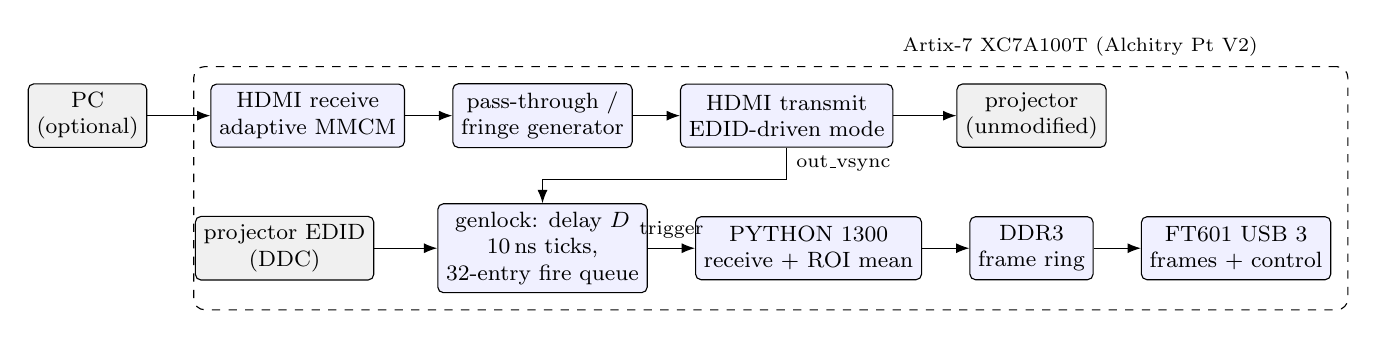
\begin{tikzpicture}[font=\footnotesize, >=Latex,
  blk/.style={draw, rounded corners=2pt, align=center, minimum height=8mm, inner sep=3pt},
  ext/.style={blk, fill=black!6}, fpga/.style={blk, fill=blue!6}]
\node[ext] (pc) {PC\\(optional)};
\node[fpga, right=8mm of pc] (rx) {HDMI receive\\adaptive MMCM};
\node[fpga, right=6mm of rx] (mux) {pass-through /\\fringe generator};
\node[fpga, right=6mm of mux] (tx) {HDMI transmit\\EDID-driven mode};
\node[ext, right=8mm of tx] (proj) {projector\\(unmodified)};
\node[fpga, below=7mm of mux] (gl) {genlock: delay $D$\\\SI{10}{\nano\second} ticks,\\32-entry fire queue};
\node[fpga, right=6mm of gl] (cam) {PYTHON 1300\\receive + ROI mean};
\node[fpga, right=6mm of cam] (ddr) {DDR3\\frame ring};
\node[fpga, right=6mm of ddr] (usb) {FT601 USB 3\\frames + control};
\node[ext, left=8mm of gl] (edid) {projector EDID\\(DDC)};
\draw[->] (pc) -- (rx); \draw[->] (rx) -- (mux); \draw[->] (mux) -- (tx); \draw[->] (tx) -- (proj);
\draw[->] (tx.south) |- node[pos=0.25, right]{\scriptsize out\_vsync} ([yshift=3mm]gl.north) -- (gl.north);
\draw[->] (gl) -- node[above]{\scriptsize trigger} (cam);
\draw[->] (cam) -- (ddr); \draw[->] (ddr) -- (usb);
\draw[->] (edid) -- (gl.west) node[midway, above]{} ;
\begin{scope}[on background layer]
\node[draw, dashed, rounded corners, fit=(rx)(mux)(tx)(gl)(cam)(ddr)(usb), inner sep=6pt,
      label={[font=\scriptsize]above right:Artix-7 XC7A100T (Alchitry Pt V2)}] {};
\end{scope}
\end{tikzpicture}
\caption{The BYOP camera. The FPGA sits on the HDMI cable; it either passes the PC's video or
replaces it with on-board fringes, and drives the projector in a mode read from the
projector's EDID. Camera triggers are timed from the \emph{output} vertical sync.
\pending{Redraw: the EDID arrow should feed the transmit side; add the UART witness.}}
\label{fig:arch}
\end{figure*}

Fig.~\ref{fig:arch} shows the device. It is built on an Alchitry Pt~V2 board with a Xilinx
Artix-7 XC7A100T and carries an ON~Semiconductor PYTHON~1300 sensor (1280$\times$1024, global
shutter, four LVDS lanes at \SI{720}{Mbps}, 10-bit) on a stacked daughter board. The HDMI
datapath is adapted from~\cite{hamsternz}; the original SLI pattern design is by Q.~Hu.

\subsection{Video path}
In pass-through, the receiver deserializes and decodes TMDS and selects the recovery clock band
from a measured input frequency, so the multiplier follows the source; a high-bandwidth MMCM
tracks spread-spectrum GPU clocks. The board reads the projector's EDID over the output DDC
channel and serves the PC a merged EDID, the intersection of the projector's modes (including
CEA-861 video data blocks) with the modes it can pass.

With no PC, the device drives the projector itself. A dedicated MMCM is retuned at run time
through its dynamic reconfiguration port and a timing generator is loaded from a table of 14
modes; the projector's EDID acts as a filter on that table, never as a source of timings, and
modes are preferred by refresh rate and then by pixel count. The fastest modes are
1280$\times$1024@60 and 800$\times$600@120 (CVT reduced blanking, \SI{73.27}{\mega\hertz}). All
results in this paper use the second.

\subsection{Pattern generator}
The fringe generator is a direct digital synthesizer whose periods adapt to the active
resolution. With $F$ the active size along the varying axis and $b=\lceil F/288\rceil$, the
three periods are $288b$, $48b$ and $8b$ pixels, an exact $1{:}6{:}36$ ratio, re-solved on
every mode change. One sequence is three frequencies $\times$ eight phases, plus a flat
full-field frame for texture. A 256-entry lookup table in the fringe path, identity at power-up,
pre-distorts the levels. For profiling, the same generator produces impulse sequences: a cycle
of five full-field frames with programmable levels (Section~\ref{sec:profiling}).

\subsection{Genlock}
The trigger is referenced to the vertical sync the device \emph{sends}, so the reference is
exact by construction. A trigger fires a programmable delay $D$ after that edge, set in
\SI{10}{\nano\second} ticks of a 24-bit time base. Because a useful delay can exceed one frame
period $T$, triggers are not single timers but entries in a 32-deep queue of absolute fire
times: every vsync enqueues one, and capture therefore advances at the full video rate whatever
$D$ is, with image $n$ holding pattern $n-\lfloor D/T\rfloor$. The device reports that offset
and whether sync is actually arriving.

Exposure is set in units of \SI{0.375}{\micro\second}. The sensor needs a readout gap between
exposures, and the firmware therefore limits the exposure to $T$ less \SI{90}{\micro\second} (an \SI{80}{\micro
\second} gap and a \SI{10}{\micro\second} margin), which at the measured
$T=\SI{8325.81}{\micro\second}$ is 21\,962 units, \SI{8235.75}{\micro\second}; a longer exposure
would halve the frame rate.

\subsection{Image and control path}
The sensor reads a full frame in a \SI{4.55}{\milli\second} burst at \SI{576}{MB/s}, faster than
USB can drain it, so frames pass through a four-slot DDR3 ring. An FT601 USB~3 bridge carries
frames and a 32-bit command channel. For
profiling, the fabric also computes the mean of a 16$\times$16 region of interest (ROI) with
counts of clipped pixels and writes it into each frame header and to an independent UART, so a
sweep needs no image transfer at all. \pending{Resource utilization of the current bitstream.}

% =====================================================================================
\section{Triggering with a Long Delay}
\label{sec:stacking}

A machine vision camera triggered through GPIO accepts a trigger only when it is ready for one,
and it reports that state on an output line; the Allied Vision Alvium~1800, for example, can
drive an output with its \texttt{FrameTriggerWait} signal, which is active while the camera
waits for a trigger \pending{cite Alvium and Basler manuals}. A trigger that arrives while the
camera is not ready, during its trigger delay or its exposure, produces no image. With a
commodity projector, the exposure for a frame must begin after the projector's input lag, which
can be longer than one frame period, and so the trigger of the next frame can arrive before the
camera is ready for it.

Let the controller send pattern $k$ with the vertical sync at time $kT$, and let the exposure
for pattern $k$ open at $kT+D$ and close at $kT+D+\tau$. For the ML750ST at \SI{120}{\hertz},
the profiled exposure has $D=\SI{8800.65}{\micro\second}$ and $\tau=\SI{6256.83}{\micro\second}$
with $T=\SI{8325.81}{\micro\second}$ (Section~\ref{sec:results}), so $D>T$: the exposure of
pattern $k$ opens after the vertical sync of pattern $k+1$.

\begin{figure}[t]
\centering
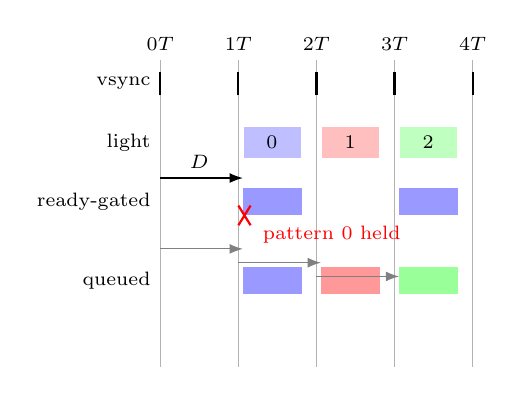
\begin{tikzpicture}[x=0.62cm, y=0.5cm, font=\scriptsize, >=Latex]
  \def\T{1.6}
  \foreach \k in {0,...,4} {
    \draw[gray!60] (\k*\T,-7.2) -- (\k*\T,0.6);
    \node[above] at (\k*\T,0.6) {$\k T$};
  }
  \node[left] at (0,0) {vsync};
  \node[left] at (0,-1.5) {light};
  \node[left] at (0,-3.0) {ready-gated};
  \node[left] at (0,-5.0) {queued};
  \foreach \k in {0,...,4} \draw[thick] (\k*\T,-0.3) -- (\k*\T,0.3);
  \foreach \k/\c in {0/blue!25,1/red!25,2/green!25} {
    \fill[\c] ({(\k+1)*\T+0.069*\T},-1.9) rectangle ({(\k+1)*\T+0.80*\T},-1.1);
    \node at ({(\k+1)*\T+0.43*\T},-1.5) {$\k$};
  }
  \fill[blue!40] ({1.057*\T},-3.35) rectangle ({1.809*\T},-2.65);
  \draw[->] (0,-2.4) -- ({1.057*\T},-2.4);
  \node[above] at ({0.5*\T},-2.4) {$D$};
  \draw[red,thick] (\T,-3.6) -- ++(0.25,0.5) (\T+0.25,-3.6) -- ++(-0.25,0.5);
  \node[red,right] at (\T+0.3,-3.85) {pattern 0 held};
  \fill[blue!40] ({2*\T+1.057*\T},-3.35) rectangle ({2*\T+1.809*\T},-2.65);
  \foreach \k/\c in {0/blue!40,1/red!40,2/green!40} {
    \fill[\c] ({\k*\T+1.057*\T},-5.35) rectangle ({\k*\T+1.809*\T},-4.65);
    \draw[->,gray] (\k*\T,{-4.2-0.35*\k}) -- ({\k*\T+1.057*\T},{-4.2-0.35*\k});
  }
\end{tikzpicture}
\caption{Triggering with a delay $D$ longer than the frame period $T$. Ready-gated: the camera is
not ready at the vertical sync of frame~1, so the controller holds pattern~0 for a second frame
and issues no trigger. Queued: every vertical sync schedules a trigger at $kT+D$, and the
pattern advances every frame. Drawn to scale for the ML750ST at \SI{120}{\hertz}
($D=1.057\,T$, $\tau=0.752\,T$).}
\label{fig:stacking}
\end{figure}

\subsection{Ready-gated triggering}
The controller of Yu \emph{et~al.}~\cite{yu2020dualprojector} connects to each external camera
through four GPIO lines: a trigger output, a camera-ready input, a mode input that selects
between pass-through and pattern generation, and an output that marks the first frame of the
pattern sequence. The controller counts the rising edges of the camera-ready input. At each
rising edge of the vertical sync, if a rising edge of camera-ready has arrived since the previous
vertical sync, the controller advances the pattern index and pulses the trigger output during the
vertical sync. If none has arrived, the controller holds the current pattern for another frame
and issues no trigger.

The trigger therefore leaves the controller at the vertical sync, and the delay $D$ is applied by
the camera, which reports ready again only after its delay and exposure have ended. A pattern is
consequently held on screen for
\begin{equation}
n_{\text{gated}} \;=\; \left\lceil \frac{D+\tau}{T} \right\rceil
\label{eq:oneshot}
\end{equation}
frames, and the fastest frame period is the trigger delay plus the exposure. For the ML750ST,
$(D+\tau)/T=1.81$, so $n_{\text{gated}}=2$: each pattern is displayed for two frames, and the
scan rate falls from \SI{120}{\hertz} to \SI{60}{\hertz}. In pass-through mode the same
handshake reaches the host, which waits for the camera to report ready before it plays the next
frame.

\subsection{Queued triggering}
The BYOP camera drives the PYTHON~1300 sensor directly, and the FPGA sets both the exposure and
the delay, so there is no ready signal to wait for. The sensor operates in pipelined global
shutter mode, integrating the next frame while it reads out the current one, and the pattern
generator advances on every vertical sync. The FPGA keeps a free-running 24-bit counter of
\SI{10}{\nano\second} ticks. At each vertical sync it writes the absolute fire time, the counter
value at that sync plus $D$, into a 32-entry first-in first-out (FIFO) queue, whether or not
earlier fire times are still waiting.

The FPGA fires the trigger at the head of the queue as soon as the counter reaches or passes its
fire time, testing the difference of the two in modular 24-bit arithmetic, so a trigger cannot be
skipped by missing an exact match. The number of triggers outstanding is counted with each push
and pop resolved in the same clock cycle, and it is reported to the host, which uses it to pair
captured images with patterns: image $n$ holds pattern $n-\lfloor D/T\rfloor$. A full queue
increments an overflow counter rather than dropping a trigger silently.

With this queue, a trigger is never withheld, and the only requirement is that one exposure and
the sensor's readout gap $g$ fit within one frame period,
\begin{equation}
\tau + g \;\le\; T,
\label{eq:stacked}
\end{equation}
which the FPGA enforces by limiting the exposure to $T$ less \SI{90}{\micro\second}, an
\SI{80}{\micro\second} gap and a \SI{10}{\micro\second} margin. The delay itself is free: $D$
may exceed several frame periods. The modular comparison is valid for delays below $2^{23}$
ticks (\SI{83.9}{\milli\second}), at which point the queue holds $\lceil D/T\rceil=11$ triggers
at \SI{120}{\hertz}, within its 32 entries. For the ML750ST, $\lceil D/T\rceil=2$ triggers are
outstanding at a time, and the scan runs at the full \SI{120}{\hertz}.
\pending{Measure: scan rate and image--pattern pairing with the queue versus ready-gated
triggering on the ML750ST.}

% =====================================================================================
\section{Profiling a Projector with a Genlocked Exposure}
\label{sec:profiling}

\subsection{Measurement model}
Let $E(t)$ be the light reaching a pixel at time $t$ after the vsync of frame~0, periodic in the
cycle length $5T$. An exposure of length $\tau$ opened at delay $d$ reads
\begin{equation}
r(d) \;=\; g\!\int_{d}^{d+\tau}\! E(t)\,dt \;+\; o \;+\; n,
\label{eq:model}
\end{equation}
with gain $g$, an offset $o$ that does not scale with $\tau$, and noise $n$. A sweep of $d$ in
steps $\le\tau$ is therefore $E$ filtered by a box of width $\tau$; we use
$\tau=\SI{4.875}{\micro\second}$ (13 units) and steps of \SI{5}{\micro\second}, 1664 delays per
frame. Each delay is held for 24 frames, the first four discarded, and the ROI mean is recorded
for every frame of the cycle, so one sweep yields all five frames at once.

\subsection{Impulse sequences}
Two five-frame sequences are swept. \emph{WKKKK} shows full white (255) in frame~0 and black in
frames~1--4; its profile is the response to one frame, and frames~2--4, far from the light,
give the camera dark level $\bar r_0$. \emph{WWWWW} shows white in every frame (254 in
frames~1--4, so that frame~0 can still be identified); its profile is the steady-state pulse
train. Since the projector re-times its input, the two are needed together: WKKKK says which
frame's light lands where, WWWWW what a continuously lit pixel sees.

\subsection{Choosing the exposure}
With $x(t)=\max(0,\,r_{\text{WKKKK}}(t)-\bar r_0)$, the fraction of one frame's light that an
exposure $[s,\,s+\tau]$ collects is
\begin{equation}
C(s,\tau) \;=\; \frac{\int_{s}^{s+\tau} x(t)\,dt}{\int_{0}^{5T} x(t)\,dt},
\qquad
C^\ast(\tau) \;=\; \max_{s}\, C(s,\tau).
\label{eq:capture}
\end{equation}
$C^\ast$ is non-decreasing in $\tau$, so the best exposure is the longest the sensor allows,
placed at the maximizing $s$. The \emph{leading} and \emph{trailing} edges of that window are the
delay $D=s$ and $s+\tau$.

\subsection{The runway}
Light can arrive before the leading edge, during the interval we call the \emph{runway}
$[\rho,\,s]$, with $\rho\ge s-T$. We place $\rho$ by walking back from $s$ while
$x(t)$ stays above \SI{2}{\percent} of its peak. Part of the runway can fall inside the
\emph{previous} exposure, which ended at $s+\tau-T$; the runway therefore splits into
\begin{equation}
\mathcal R_1=[\rho,\; s+\tau-T], \qquad \mathcal R_2=[s+\tau-T,\; s],
\end{equation}
the part inside the previous exposure and the part between exposures.

\subsection{Leakage maps}
To see whose light arrives in each part, the generator switches to a two-frame cycle
$A\,B\,A\,B$ of full-field levels. A reading in a window of frame $k$ then sees that frame's
level $x$ and the level $y$ of frames $k\pm1$, which are equal. Sweeping all
$(A,B)$ pairs, each giving the two mirrored cells $(y,x)=(B,A)$ and $(A,B)$, fills a
$256\times256$ map $M_i(y,x)$ for each window $\mathcal R_i$, the exposure opened at the
window's start and lasting its length, 10 readings per cell. A map that varies with $y$ shows
light from the neighbouring patterns; one that varies with $x$ shows light from the runway's own
frame. The A--B--A--B cycle cannot tell the previous pattern from the next one; separating
them needs a longer cycle. \pending{Three-frame cycle to break the ambiguity.}

\subsection{Colour decomposition}
WWWWW is repeated through red, green and blue filters on the camera. With
$w(t)$ and $f_c(t)$ the white and filtered sweeps less $\bar r_0$, we fit
\begin{equation}
w(t) \;\approx\; \sum_{c\in\{R,G,B\}} a_c\, f_c(t) + b
\label{eq:rgbfit}
\end{equation}
by least squares over every delay. The weights absorb the filters' transmission; the
fitted terms $a_c f_c(t)$ are the per-LED pulse trains of white, and the residual shows
whatever white contains that the three filtered sweeps do not.

% =====================================================================================
\section{Experiments}
\label{sec:results}

\paragraph*{Setup}
The projector is an Optoma ML750ST LED DLP driven by the device at 800$\times$600@120 with no PC
(on this model \SI{120}{\hertz} enables its 3D mode). The sensor, without a lens, sits on the
projection lens axis about \SI{17}{\milli\metre} in front of the lens in a printed cap, so it
sees light only when an LED is on and the corresponding mirrors are in the on state; a lens iris
on the cap keeps the peak below clipping, and filters fit in front of it. The ROI is the
16$\times$16 patch at the sensor centre. The measured period is
$T=\SI{8325.81}{\micro\second}$; the vsync-to-first-active-line time is
\SI{432.0}{\micro\second}. All sweeps are from one profiling session saved as a single document
(19 Oct 2026); every number below is printed by the figure script from that document.

\subsection{Latency and pulse train}

\begin{figure*}[t]
\centering
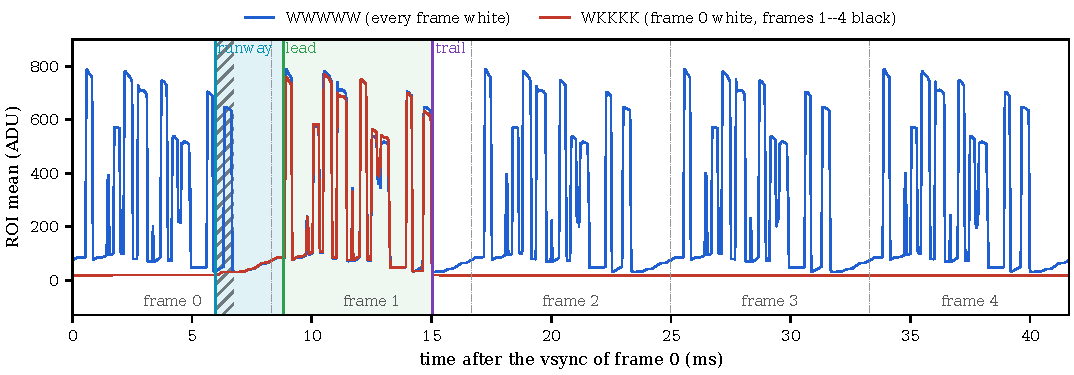
\includegraphics[width=\textwidth]{figures/timeline.pdf}
\caption{Five-frame profiles of the ML750ST at 800$\times$600@120 (exposure
\SI{4.875}{\micro\second}, step \SI{5}{\micro\second}, ROI mean). The light of the white frame~0
(red, WKKKK) appears in frame~1: the projector is one frame late. Blue (WWWWW) is the
steady-state pulse train. Shaded: the chosen exposure (lead to trail) and the runway before it;
hatched: the part of the runway inside the previous exposure.}
\label{fig:timeline}
\end{figure*}

Fig.~\ref{fig:timeline} shows both sequences. The white frame's light falls in frame~1: the
projector delays its input by exactly one frame. Within a frame the light is a train of separate
pulses; the WKKKK pulses in frame~1 and the WWWWW pulses in any frame coincide, with a median
ratio of 1.009 between them in lit slices. The camera dark level is $\bar r_0=18.33$~ADU. The
WWWWW profile never returns to it (minimum 30.25~ADU), so with a continuously lit picture there
is no dark interval anywhere in the frame.

\subsection{Exposure window}

\begin{figure}[t]
\centering
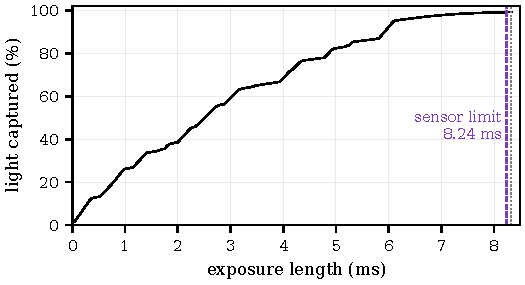
\includegraphics[width=\columnwidth]{figures/captured_vs_exposure.pdf}
\caption{Best fraction of a frame's light captured, $C^\ast(\tau)$ of~\eqref{eq:capture}, against
exposure length, from the WKKKK profile. The sensor's limit at this frame rate is
\SI{8235.75}{\micro\second}.}
\label{fig:capture}
\end{figure}

Fig.~\ref{fig:capture} plots $C^\ast(\tau)$. A \SI{2}{\milli\second} exposure collects at best
\SI{38.6}{\percent} of a frame's light, \SI{4}{\milli\second} \SI{68.5}{\percent} and
\SI{6}{\milli\second} \SI{92.3}{\percent}. The edges saved in the session,
$s=\SI{8800.65}{\micro\second}$ and $s+\tau=\SI{15057.48}{\micro\second}$
($\tau=\SI{6256.83}{\micro\second}$), collect \SI{95.6}{\percent}; the runway holds
\SI{4.0}{\percent} and everything else \SI{0.04}{\percent}. At the sensor's limit the best
window collects \SI{99.2}{\percent}. \pending{Decide which exposure the 3D experiments use and
re-save the edges at the limit if so.}

\subsection{LED decomposition}

\begin{figure*}[t]
\centering
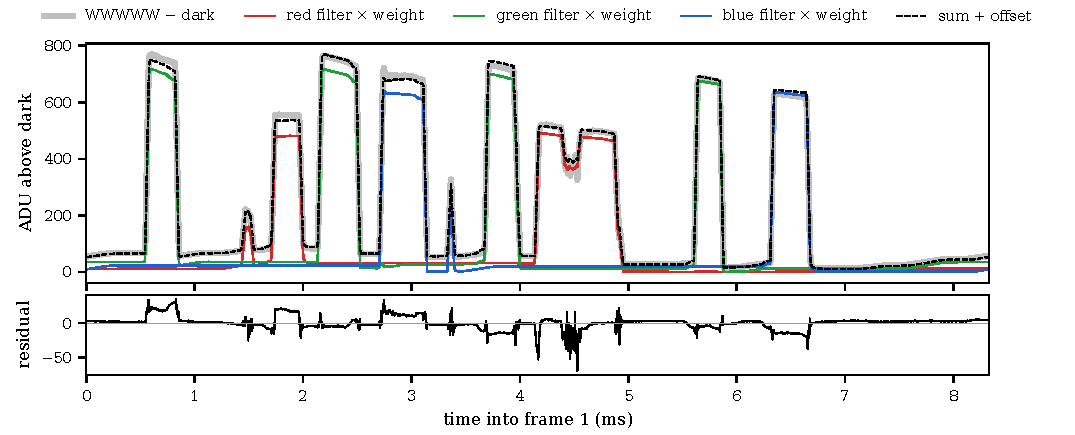
\includegraphics[width=\textwidth]{figures/rgb_fit.pdf}
\caption{White (grey band, WWWWW less dark) as a weighted sum of red-, green- and
blue-filtered sweeps~\eqref{eq:rgbfit}, one frame. Bottom: residual.}
\label{fig:rgb}
\end{figure*}

The least-squares weights of~\eqref{eq:rgbfit} are $a_R=0.4935$, $a_G=1.2192$, $a_B=0.6945$ and
$b=-3.28$~ADU; the residual is 9.61~ADU RMS against a 771.7~ADU peak, $R^2=0.99880$
(Fig.~\ref{fig:rgb}). Of the fitted light, red carries \SI{27.4}{\percent}, green
\SI{44.7}{\percent} and blue \SI{27.8}{\percent}. Folded onto one frame and thresholded at
\SI{25}{\percent}, the pulses are red at 1450--1535, 1715--1995 and
\SIrange{4150}{4940}{\micro\second}; green at 555--850, 2145--2520,
3685--3975 and \SIrange{5620}{5870}{\micro\second}; and blue at
2715--3135 and \SIrange{6320}{6675}{\micro\second}, with a short blue flash near
\SI{3367}{\micro\second}. No two colours are lit at once, and some LED is lit in
\SI{37.8}{\percent} of the frame. The largest residuals sit on pulse edges (largest
70.6~ADU), where a small timing difference between sweeps leaves a spike, and inside the long
red pulse. \pending{Red sweep may be partly clipped (143 readings $\ge$1000~ADU); re-run with the
iris closed a step.}

\subsection{Leakage before the exposure}

\begin{figure*}[t]
\centering
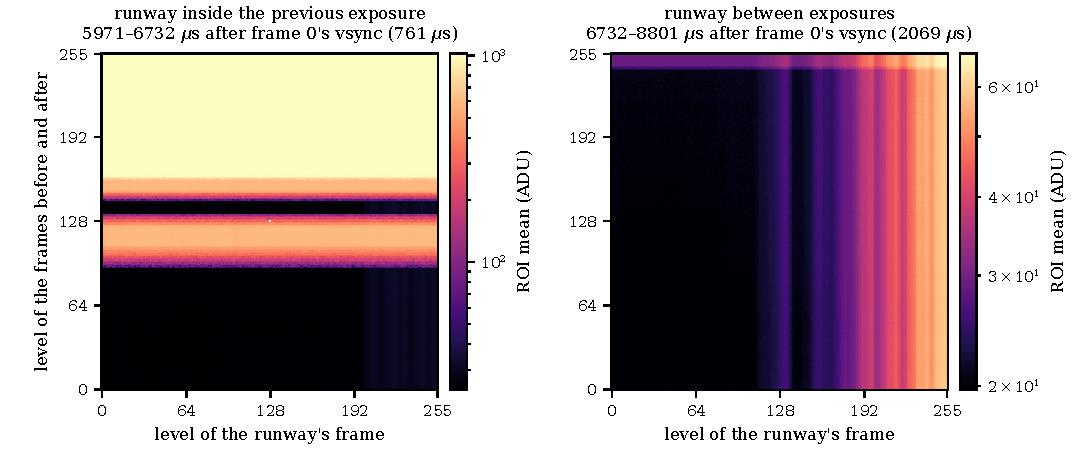
\includegraphics[width=\textwidth]{figures/runway_maps.pdf}
\caption{Leakage maps for the two parts of the runway (A\,B\,A\,B cycle, all $256\times256$
level pairs, 10 readings per cell; log colour). Left: inside the previous exposure,
\SI{760.5}{\micro\second} exposure. Right: between exposures, \SI{2068.9}{\micro\second}.}
\label{fig:runway}
\end{figure*}

The runway of the saved edges runs from $\rho=\SI{5970.99}{\micro\second}$ to $s$; the previous
exposure ended at $s+\tau-T=\SI{6731.67}{\micro\second}$, so $\mathcal R_1$ is
\SI{760.7}{\micro\second} long and $\mathcal R_2$ \SI{2069.0}{\micro\second}. They hold
\SI{0.35}{\percent} and \SI{3.65}{\percent} of the white frame's light.

The two maps in Fig.~\ref{fig:runway} behave differently. In $\mathcal R_1$ the reading is set
almost entirely by the level of the neighbouring frames $y$: a linear fit in $x$ alone explains
none of the variance, and the full range of the map, 24 to beyond 1023~ADU, is crossed by
changing $y$. The dependence on $y$ is not monotonic: about 24~ADU up to $y\approx88$, a band
near $y=96$--$120$, a return to the floor near $y=136$, and saturation from about $y=164$.
\pending{Interpret: consistent with the bit-plane order of the last LED pulse
(\SIrange{6320}{6675}{\micro\second}, blue); test with filtered maps.} In $\mathcal R_2$ the
reading is set by the runway frame's own level $x$: from \SI{20.0}{} to \SI{57.2}{ADU} across $x$
at $y=0$ ($R^2=0.694$ for a linear fit in $x$, 0.005 in $y$), with a step of about 9~ADU only
when $y\gtrsim244$.

Read with the one-frame latency, the first map is light of the \emph{previous} pattern, which
the previous exposure is meant to collect and the current one must not, while the second is
early light that tracks the pattern about to be captured. An exposure may therefore be extended
backwards into $\mathcal R_2$ at the cost of a level-dependent but self-consistent bias, but not
into $\mathcal R_1$. \pending{Confirm with a three-frame cycle; quantify the phase error each
would introduce.}

% =====================================================================================
\section{Implications for Structured Light}
\label{sec:sli}

\pending{PLANNED EXPERIMENTS, no results yet.
(1) Phase error on a flat target with the 24-frame sequence, for exposures placed naively
(delay 0), at the profiled window of 6257\,\textmu s, and at the sensor limit.
(2) The same with a per-pixel leakage correction derived from the maps.
(3) Depth RMS on calibrated planes and a sphere; comparison with a PC-driven projector and a
free-running camera.
(4) Several projectors (DLP LED, DLP lamp with colour wheel, LCD) to show the profiling
generalizes.
(5) Frame rate and latency of the full 3D pipeline.}

% =====================================================================================
\section{Limitations}
\label{sec:limits}
The profiles are ROI means over a 16$\times$16 patch with the sensor at the lens, not images of
a scene; a pixel in a scanned scene integrates the same pulse train through a different optical
path. The A\,B\,A\,B cycle confounds the
previous and the next pattern. One projector has been measured.

% =====================================================================================
\section{Conclusion}
\label{sec:conclusion}
Putting the camera inside the HDMI path turns an unmodified projector into an instrument whose
timing can be measured rather than assumed. The same genlocked exposure that captures
structured light, stepped through an impulse sequence, recovers the projector's latency, its LED
pulse train, an exposure window that collects nearly all of a frame's light, and the light that
leaks into that window from neighbouring patterns. \pending{Summarize the 3D results.}

\section*{Acknowledgments}
The HDMI datapath derives from M.~Field's Artix-7 HDMI processing design~\cite{hamsternz}; the
original SLI design is by Q.~Hu. \pending{Funding.}

\bibliographystyle{IEEEtran}
\bibliography{refs}

\end{document}
